\documentclass[a4paper]{article}
\usepackage[14pt]{extsizes} % для того чтобы задать нестандартный 14-ый размер шрифта
\usepackage[utf8]{inputenc}
\usepackage[russian]{babel}
\usepackage{setspace,amsmath}
\usepackage{graphicx}
\usepackage[left=20mm, top=15mm, right=15mm, bottom=15mm, nohead, footskip=10mm]{geometry} % настройки полей документа
 
\begin{document} % начало документа
 % НАЧАЛО ТИТУЛЬНОГО ЛИСТА
\begin{center}
\hfill \break
\large{Министерство образования и науки РФ}\\
\large{ФЕДЕРАЛЬНОЕ ГОСУДАРСТВЕННОЕ БЮДЖЕТНОЕ ОБРАЗОВАТЕЛЬНОЕ УЧРЕЖДЕНИЕ}\\ 
\large{ВЫСШЕГО ОБРАЗОВАНИЯ}\\
\large{НАЦИОНАЛЬНЫЙ ИССЛЕДОВАТЕЛЬСКИЙ УНИВЕРСИТЕТ «МЭИ»}\\
\hfill \break
\normalsize{Прикладная математика и информатика}\\
 \hfill \break
\normalsize{Кафедра прикладной математики и искусственного интеллекта}\\
\hfill\break
\hfill \break
\hfill \break
\hfill \break
\large{Теоретические модели вычисления}\\
\hfill \break
\large{Домашнее задание №1}\\
\large{Регулярные языки и конечные автоматы}\\
\hfill \break
\hfill \break
\hfill \break
\hfill \break
\hfill \break
\hfill \break
\end{center}
 
\normalsize{ 
\begin{flushright}
\ Преподаватель: Ивлиев С.А. \\
\ Студент: Соколова А.С. \
\end{flushright}
\hfill \break
\hfill \break
\hfill \break
\hfill \break
\hfill \break
\begin{center} Москва 2022 \end{center}
\thispagestyle{empty} % выключаем отображение номера для этой страницы
} 
% КОНЕЦ ТИТУЛЬНОГО ЛИСТА

% СОДЕРЖАНИЕ
\newpage
    \tableofcontents % Вывод содержания
\newpage
% КОНЕЦ СОДЕРЖАНИЯ 
 
% ЗАДАНИЕ 1
\newpage
\section{Задание №1. Построить конечный автомат, распознающий языык.}
\begin{enumerate}
\item {$L = \{ w \in \{a,b,c\}*$ | $  {|w|_c} = 1 \} $}\\
\begin{figure}[h]
\centering
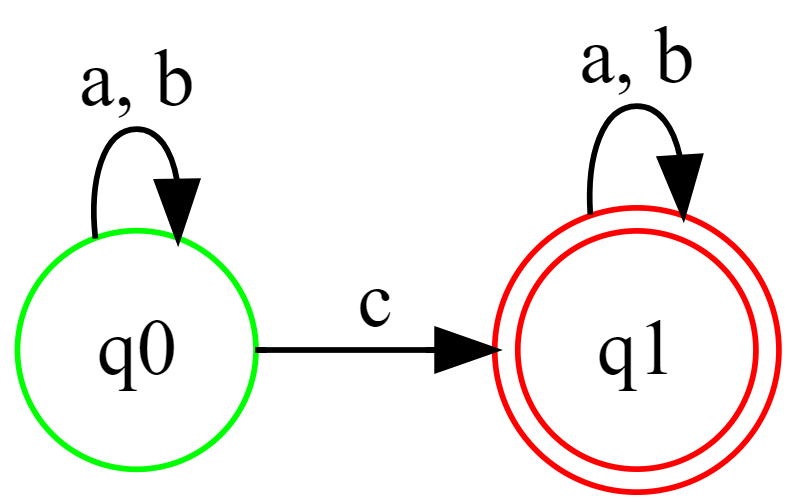
\includegraphics[width=7cm]{Задание_№1_1.png}
\end{figure}

\item {$L = \{ w \in \{a,b\}*$ | $  {|w|_a} \le 2, {|w|_b} \ge 2 \}$}\\ 
\ У нас может быть 1 или 2 буквы а и бесконечное число букв b, начиная с двух\\
\ Примерные варианты: bb..aa; bab..ba; bab..ab;ab..ab; ab..bb;  и т д  \\
\begin{figure}[h]
\centering
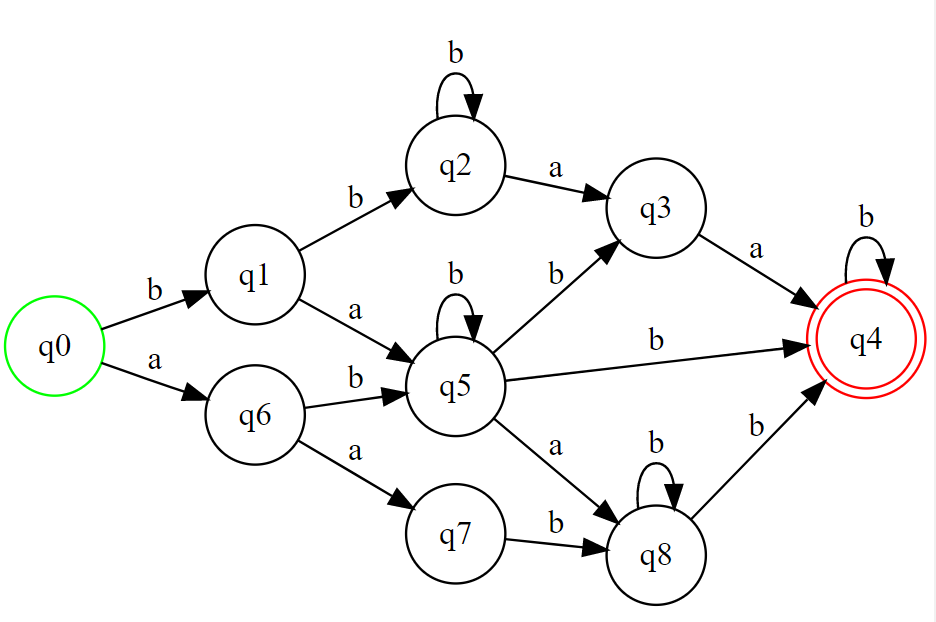
\includegraphics[width=18cm]{Задание_№1_2.png}
\end{figure}
\\Проверим через прямое произведение\\

Построим сначала автомат:\\
$L_1_1 = \{ w \in \{a,b\}  $ | $  {|w|_a} \le 2 \} $\\
\begin{figure}[h]
\centering
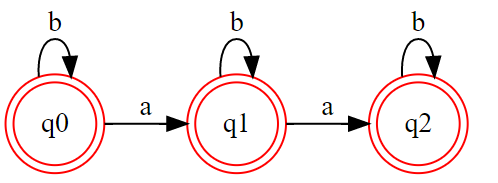
\includegraphics[width=12cm]{Задание_№1_1_2.png}
\end{figure}
\\Потом автомат:\\
$L_1_2 = \{ w \in \{a,b\}  $ | $  {|w|_b} \ge 2 \} $
\begin{figure}[h]
\centering
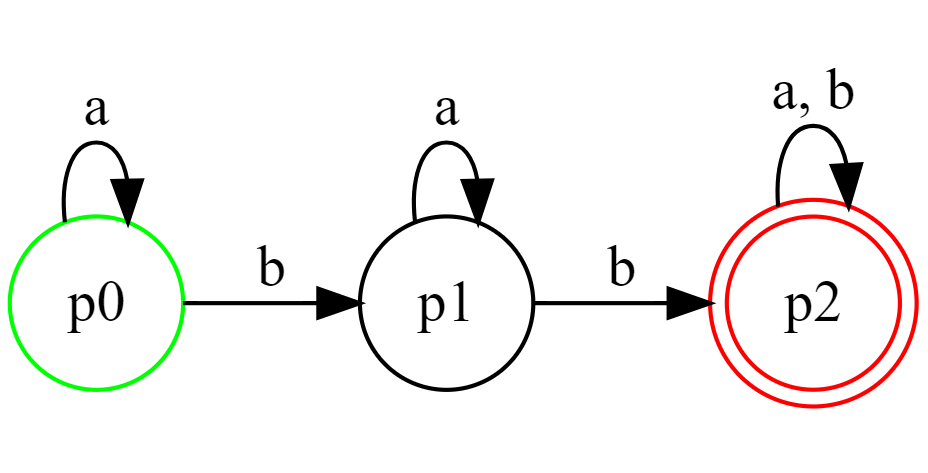
\includegraphics[width=12cm]{Задание_№2_1_1.png}
\end{figure}

\\Найдем ппрямое произведение $L_1_1$ \cap $L_1_2$.
\\где  $A_1_1 = (\sum_1 , Q_1, s_1, T_1, \delta_1) $ и  $A_1_2 = (\sum_2 , Q_2, s_2, T_2, \delta_2)$:\\
\hfill \break
$\sum = \sum_1 \bigcup \sum_2 = \{a, b\}$\\
$Q = Q_1 \times Q_2$ $= \{q0p0, q0p1, q0p2, q1p0, q1p1, q1p2, q2p0, q2p1, q2p2 \}$\\
$s = <s_1, s_2> = q0p0$\\
$T = T_1 \times T_2 = q2p2, q1p2, q0p2$\\
$ \delta(<q1, q2>, c) = <\delta_1(q_1, c), \delta_2(q_2, c)>$\\ Распишем все $\delta$ \\
$\delta(q0p0, a) = q1p0$ \ $\delta(q0p0, b) = q0p1$ \\
$\delta(q0p1, a) = q1p1$ \ $\delta(q0p1, b) = q0p2$ \\
$\delta(q0p2, a) = q1p2$ \ $\delta(q0p2, b) = q0p2$ \\
$\delta(q1p0, a) = q2p0$ \ $\delta(q1p0, b) = q1p1$ \\
$\delta(q1p1, a) = q2p1$ \ $\delta(q1p1, b) = q1p2$ \\
$\delta(q1p2, a) = q2p2$ \ $\delta(q1p2, b) = q1p2$ \\
$\delta(q2p0, a) = -$ \ \ \ \ \ $\delta(q2p0, b) = q2p1$ \\
$\delta(q2p1, a) = -$ \ \ \ \ \ $\delta(q2p1, b) = q2p2$ \\
$\delta(q2p2, a) = -$ \ \ \ \ \ $\delta(q2p2, b) = q2p2$ \\
Построем автомат:\\
\begin{figure}[h]
\centering
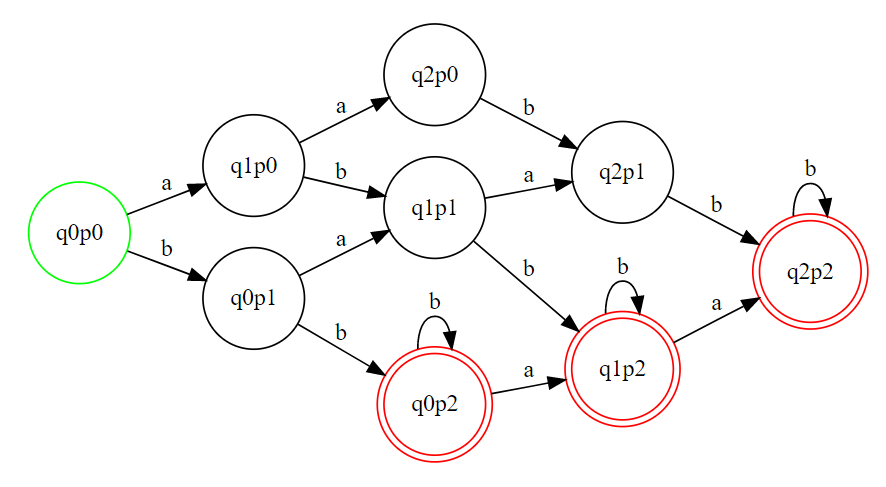
\includegraphics[width=18cm]{Задание_№1_1_3.png}
\end{figure}
\\Заметим, что автоматы не совпадают. Ответом является второй автомат, построенный через прямое произведение
\item {$L = \{ w \in \{a,b\}*$ | $  {|w|_a} \ne {|w|_b}  \}$} \\


\item {$L = \{ w \in \{a,b\}*$ | $  {ww = www} \}$} \\
Здесь могут быть только пустые слова 
\begin{figure}[h]
\centering
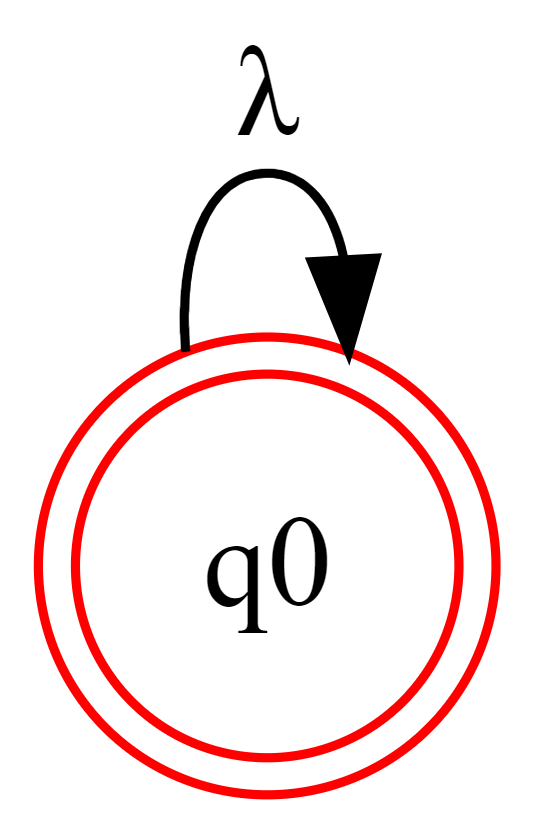
\includegraphics[width=4cm]{Задание_№1_4.png}
\end{figure}
\end{enumerate}
\newpage
% КОНЕЦ ЗАДАНИЯ 1


% ЗАДАНИЕ 2
\newpage
\section{Задание №2. Построить конечный автомат, используя прямое произведение.}
\begin{enumerate}
\item {$L_1 = \{ w \in \{a,b\}  $ | $  {|w|_a} \ge 2  \wedge   {|w|_b} \ge 2 \} $}\\
Построим сначала автомат: 
$L_1_1 = \{ w \in \{a,b\}  $ | $  {|w|_a} \ge 2 \} $
\begin{figure}[h]
\centering
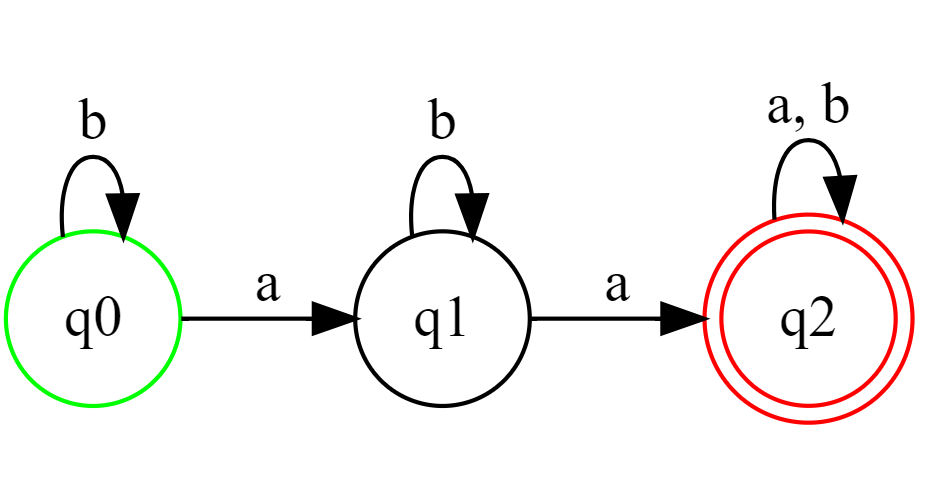
\includegraphics[width=12cm]{Задание_№2_1_2.png}
\end{figure}
\\Потом автомат:
$L_1_2 = \{ w \in \{a,b\}  $ | $  {|w|_b} \ge 2 \} $
\begin{figure}[h]
\centering
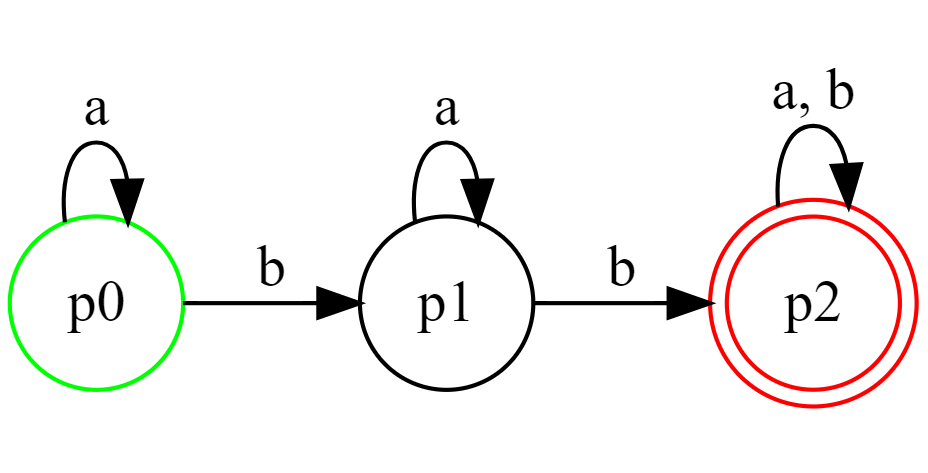
\includegraphics[width=12cm]{Задание_№2_1_1.png}
\end{figure}
\\Найдем ппрямое произведение $L_1_1$ \cap $L_1_2$.
\\где  $A_1_1 = (\sum_1 , Q_1, s_1, T_1, \delta_1) $ и  $A_1_2 = (\sum_2 , Q_2, s_2, T_2, \delta_2)$:\\
\hfill \break
$\sum = \sum_1 \bigcup \sum_2 = \{a, b\}$\\
$Q = Q_1 \times Q_2$ $= \{q0p0, q0p1, q0p2, q1p0, q1p1, q1p2, q2p0, q2p1, q2p2 \}$\\
$s = <s_1, s_2> = q0p0$\\
$T = T_1 \times T_2 = q2p2$\\
$ \delta(<q1, q2>, c) = <\delta_1(q_1, c), \delta_2(q_2, c)>$\\ Распишем все $\delta$ \\
$\delta(q0p0, a) = q1p0$ \  $\delta(q0p0, b) = q0p1$ \\
$\delta(q0p1, a) = q1p1$ \  $\delta(q0p1, b) = q0p2$ \\
$\delta(q0p2, a) = q1p2$ \  $\delta(q0p2, b) = q0p2$ \\
$\delta(q1p0, a) = q2p0$ \  $\delta(q1p0, b) = q1p1$ \\
$\delta(q1p1, a) = q2p1$ \  $\delta(q1p1, b) = q1p2$ \\
$\delta(q1p2, a) = q2p2$ \  $\delta(q1p2, b) = q1p2$ \\
$\delta(q2p0, a) = q2p0$ \  $\delta(q2p0, b) = q2p1$ \\
$\delta(q2p1, a) = q2p1$ \  $\delta(q2p1, b) = q2p2$ \\
$\delta(q2p2, a) = q2p2$ \  $\delta(q2p2, b) = q2p2$ \\
Построим автомат:\\
\begin{figure}[h]
\centering
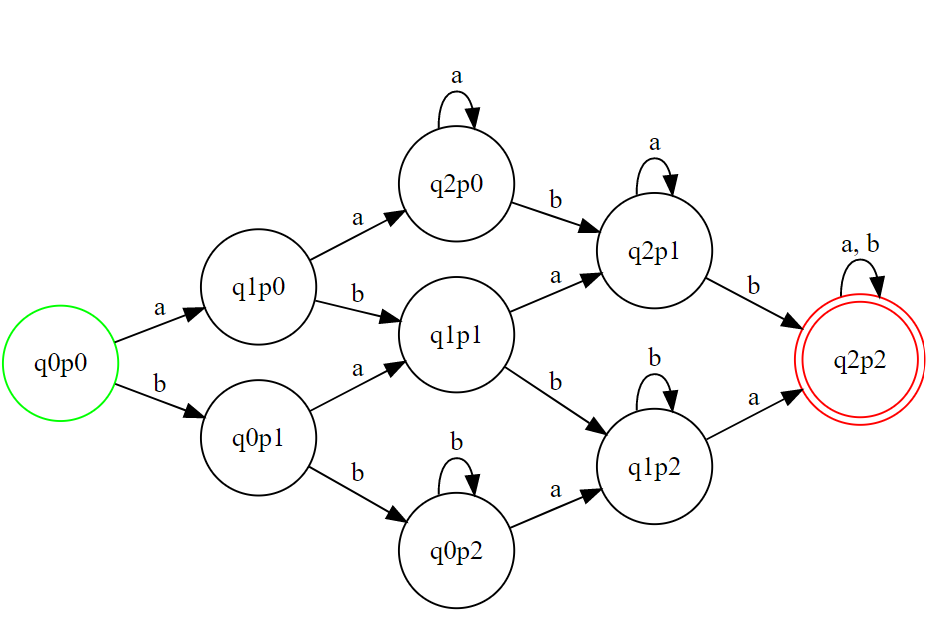
\includegraphics[width=18cm]{Задание_№2_1_3.png}
\end{figure}


\item {$L_2 = \{ w \in \{a,b\}*$ | $  {|w|} \ge 3 \wedge {|w|} $ нечётное $ \} $}\\


Построим сначала автомат: 
$L_1_1$ = \{$ w \in \{a,b\}*   $|$  {|w|} \ge 3 $ \} \\
\begin{figure}[h]
\centering
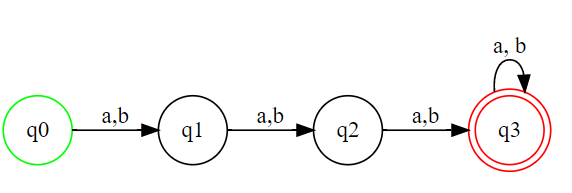
\includegraphics[width=15cm]{Задание_№2_2_1.png}
\end{figure}
\\Потом автомат:
$L_1_2$ = \{$ w \in \{a,b\}*   $|$  {|w|} $ нечётное $ $ \} \\
Количество вхождений a или b в слово w должно быть нечетным.

\begin{figure}[h]
\centering
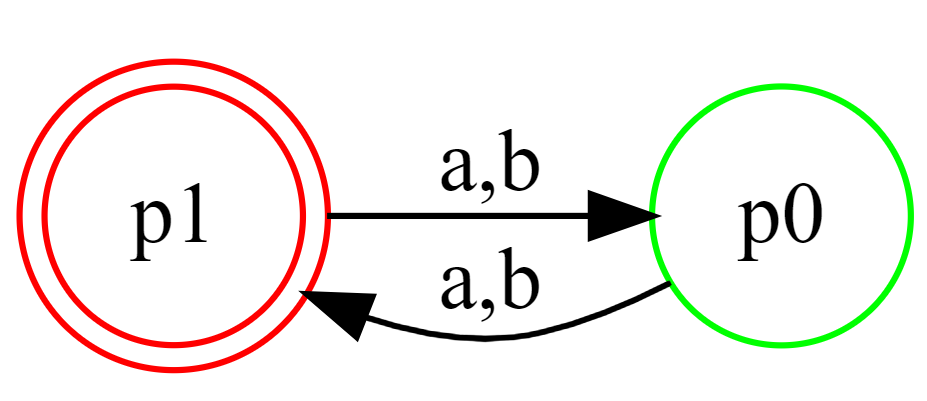
\includegraphics[width=7cm]{Задание_№2_2_2.png}
\end{figure}

\\Найдем прямое произведение $L_1_1$ \cap $L_1_2$.
\\где  $A_1_1 = (\sum_1 , Q_1, s_1, T_1, \delta_1) $ и  $A_1_2 = (\sum_2 , Q_2, s_2, T_2, \delta_2)$:\\
\hfill \break
$\sum = \sum_1 \bigcup \sum_2 = \{a, b\}$\\
$Q = Q_1 \times Q_2$ $= \{q0p0, q0p1, q1p0, q1p1, q2p0, q2p1, q3p0, q3p1 \}$\\
$s = <s_1, s_2> = q0p0$\\
$T = T_1 \times T_2 = q3p1$\\
$ \delta(<q1, q2>, c) = <\delta_1(q_1, c), \delta_2(q_2, c)>$\\ Распишем все $\delta$ \\
$\delta(q0p0, a) = q1p1$ \  $\delta(q0p0, b) = q1p1$ \\
$\delta(q0p1, a) = q1p0$ \  $\delta(q0p1, b) = q1p0$ \\
$\delta(q1p0, a) = q2p1$ \  $\delta(q1p0, b) = q2p1$ \\
$\delta(q1p1, a) = q2p0$ \  $\delta(q1p1, b) = q2p0$ \\
$\delta(q2p0, a) = q3p1$ \  $\delta(q2p0, b) = q3p1$ \\
$\delta(q2p1, a) = q3p0$ \  $\delta(q2p1, b) = q3p0$ \\
$\delta(q3p0, a) = q3p1$ \  $\delta(q3p0, b) = q3p1$ \\
$\delta(q3p1, a) = q3p0$ \  $\delta(q3p1, b) = q3p0$ \\

Построим автомат:\\
\begin{figure}[h]
\centering
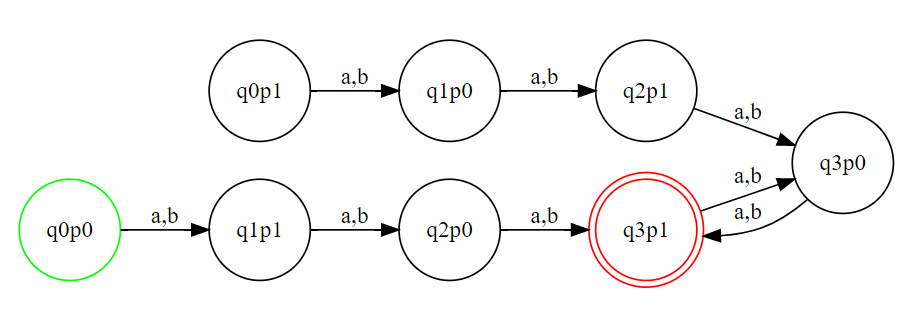
\includegraphics[width=18cm]{Задание_№2_2_3.png}
\end{figure}


\item {$L_3$ = \{ $w$ \in \{$a,b$\}$*$ $|$  $ {|w|_a}$ чётно  $\wedge$ ${|w|_b}$ кратно трём \} }\\
Построим сначала автомат: 
$L_1_1$ = \{$ w \in \{a,b\}*   $|$  {|w|_a} $чётно$ $ \} \\
\begin{figure}[h]
\centering
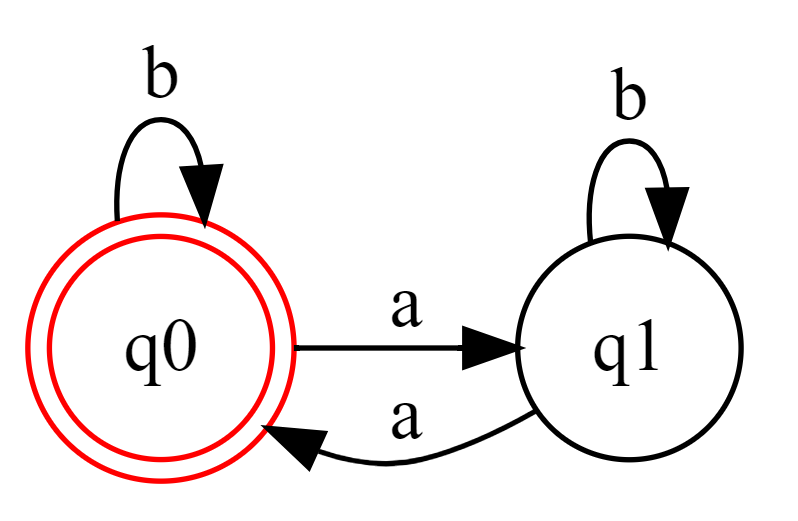
\includegraphics[width=8cm]{Задание_№2_3_1.png}
\end{figure}
\\
\\Потом автомат:
$L_1_2$ = \{$ w \in \{a,b\}*   $|$  {|w|_b} $ кратно трём $ $ \} \\
\begin{figure}[h]
\centering
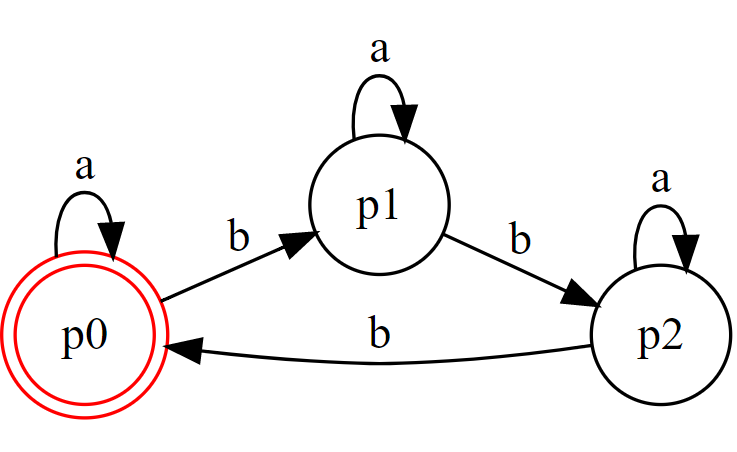
\includegraphics[width=9cm]{Задание_№2_3_2.png}
\end{figure}

\\Найдем прямое произведение $L_1_1$ \cap $L_1_2$.
\\где  $A_1_1 = (\sum_1 , Q_1, s_1, T_1, \delta_1) $ и  $A_1_2 = (\sum_2 , Q_2, s_2, T_2, \delta_2)$:\\
\hfill \break
$\sum = \sum_1 \bigcup \sum_2 = \{a, b\}$\\
$Q = Q_1 \times Q_2$ $= \{q0p0, q0p1, q0p2, q1p0, q1p1, q1p2 \}$\\
$s = <s_1, s_2> = q0p0$\\
$T = T_1 \times T_2 = q0p0$\\
$ \delta(<q1, q2>, c) = <\delta_1(q_1, c), \delta_2(q_2, c)>$\\ 
\\Распишем все $\delta$ \\ \\
$\delta(q0p0, a) = q1p0$ \  $\delta(q0p0, b) = q0p1$ \\
$\delta(q0p1, a) = q1p1$ \  $\delta(q0p1, b) = q0p2$ \\
$\delta(q0p2, a) = q1p2$ \  $\delta(q0p2, b) = q0p0$ \\
$\delta(q1p0, a) = q0p0$ \  $\delta(q1p0, b) = q1p1$ \\
$\delta(q1p1, a) = q0p1$ \  $\delta(q1p1, b) = q1p2$ \\
$\delta(q1p2, a) = q0p2$ \  $\delta(q1p2, b) = q1p0$ \\

\\Построим автомат:\\
\begin{figure}[h]
\centering
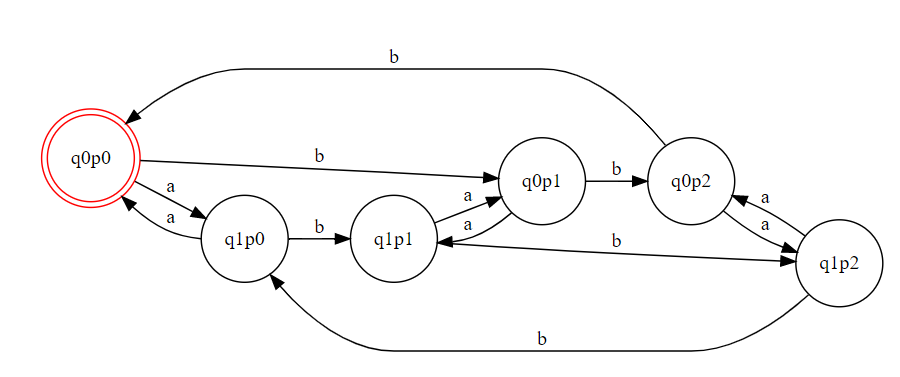
\includegraphics[width=18cm]{Задание_№2_3_3.png}
\end{figure}


\item {$L_4$ = $\overline{L_3}$}\\


\item {$L_5 = L_2 \setminus L_3 $}\\
\end{enumerate}
\newpage
% КОНЕЦ ЗАДАНИЯ 2



\end{document}  % КОНЕЦ ДОКУМЕНТА !